%%%%%%%%%%%%%%%%%%%%%%%%%%%%%%%%%%%%%%%%%%%%%%%%%%%%%%%%%%%%%%%
%
% Welcome to writeLaTeX --- just edit your LaTeX on the left,
% and we'll compile it for you on the right. If you give
% someone the link to this page, they can edit at the same
% time. See the help menu above for more info. Enjoy!
%
%%%%%%%%%%%%%%%%%%%%%%%%%%%%%%%%%%%%%%%%%%%%%%%%%%%%%%%%%%%%%%%

% --------------------------------------------------------------
% This is all preamble stuff that you don't have to worry about.
% Head down to where it says "Start here"
% --------------------------------------------------------------
 
\documentclass[12pt]{report}
 
\usepackage[margin=1in]{geometry}
\usepackage{amsmath,amsthm,amssymb}
\usepackage{hyperref}
\usepackage[nottoc,numbib]{tocbibind}
\usepackage{graphicx}
\graphicspath{{./images/}}

\usepackage{tikz}
\usetikzlibrary{shapes,positioning}

\tikzset{ell/.style={circle,draw,minimum height=0.5cm,minimum width=0.5cm,inner sep=0.2cm}}
\tikzset{rec/.style={rectangle,draw,minimum height=0.5cm,minimum width=0.5cm,inner sep=0.2cm}}

\usepackage{listings}
\usepackage{xcolor}

%New colors defined below
\definecolor{codegreen}{rgb}{0,0.6,0}
\definecolor{codegray}{rgb}{0.5,0.5,0.5}
\definecolor{codepurple}{rgb}{0.58,0,0.82}
\definecolor{backcolour}{rgb}{0.95,0.95,0.92}

%Code listing style named "mystyle"
\lstdefinestyle{mystyle}{
  backgroundcolor=\color{backcolour}, commentstyle=\color{codegreen},
  keywordstyle=\color{magenta},
  numberstyle=\tiny\color{codegray},
  stringstyle=\color{codepurple},
  basicstyle=\ttfamily\footnotesize,
  breakatwhitespace=false,         
  breaklines=true,                 
  captionpos=b,                    
  keepspaces=true,                 
  numbers=left,                    
  numbersep=5pt,                  
  showspaces=false,                
  showstringspaces=false,
  showtabs=false,                  
  tabsize=2
}

%"mystyle" code listing set
\lstset{style=mystyle}

 
\newcommand{\N}{\mathbb{N}}
\newcommand{\Z}{\mathbb{Z}}
 
\newenvironment{theorem}[2][Theorem]{\begin{trivlist}
\item[\hskip \labelsep {\bfseries #1}\hskip \labelsep {\bfseries #2.}]}{\end{trivlist}}
\newenvironment{lemma}[2][Lemma]{\begin{trivlist}
\item[\hskip \labelsep {\bfseries #1}\hskip \labelsep {\bfseries #2.}]}{\end{trivlist}}
\newenvironment{exercise}[2][Exercise]{\begin{trivlist}
\item[\hskip \labelsep {\bfseries #1}\hskip \labelsep {\bfseries #2.}]}{\end{trivlist}}
\newenvironment{problem}[2][Problem]{\begin{trivlist}
\item[\hskip \labelsep {\bfseries #1}\hskip \labelsep {\bfseries #2.}]}{\end{trivlist}}
\newenvironment{question}[2][Question]{\begin{trivlist}
\item[\hskip \labelsep {\bfseries #1}\hskip \labelsep {\bfseries #2.}]}{\end{trivlist}}
\newenvironment{corollary}[2][Corollary]{\begin{trivlist}
\item[\hskip \labelsep {\bfseries #1}\hskip \labelsep {\bfseries #2.}]}{\end{trivlist}}

\newenvironment{solution}{\begin{proof}[Solution]}{\end{proof}}
 
\begin{document}
 
% --------------------------------------------------------------
%                         Start here
% --------------------------------------------------------------
 
\title{Texas A\&M University Kingsville\\
Department of EECS\\
CSEN 5303 Foundations of Computer Science\\
Project 4 Multi Stack
}%Institution, Department
\author{\\
Mengxiang Jiang\\ %replace with your name
Professor Habib Ammari} %if necessary, replace with your course title
 
\maketitle

\tableofcontents

\chapter{Introduction}
The problem given is to store $k$ stacks in a single array such that when one stack grows
to the boundary of another stack, we will need to reorganize the stacks so all the stack have size proportional gaps between them.
The problem is split into 4 questions which are listed below and answered in the Design chapter:

\begin{enumerate}
    \item On the assumption that there is a procedure $reorganize$ to call when stacks collide, write
    code for the five stack operations. 
    \item On the assumption that there is a procedure $MakeNewTops$ that computes $newtop[i]$, the
    ``appropriate" position for the top of stack i, for $1 \leq i \leq k$, write the procedure $reorganize$.
    \item What is an appropriate implementation for the goal stack in (2)? Do we really need to keep
    it as a list of integers, or will a more succinct representation do?
    \item Implement $MakeNewTops$ in such a way that space above each stack is proportional to the
    current size of that stack. 
\end{enumerate}

The implementation of this multi-stack structure is in Python.

\chapter{Design}
\label{chapter:design}
For the first question, here is the pseudocode for each of the five stack operations
under the assumption that there is a $reorganize$ procedure:
\begin{verbatim}
type
    MultiStack = record
        stk_size, arr_size: integer;
        tops, bots: array[0..stk_size-1] of integer;
        arr: array[0..arr_size-1] of elementtype;
    end;

procedure Push(snum: integer, elem: elementtype; var MS: MultiStack);
    begin
        if IsFull(MS) then
            error('stack is full');
        else if (snum < MS.stk_size - 1) and 
        (MS.tops[snum]+1 = MS.bots[snum+1]) then begin
            reorganize(MS);
            Push(snum, elem, MS);
        end;
        else begin
            MS.tops[snum] := MS.tops[snum] + 1;
            MS.arr[MS.tops[snum]] := elem;
        end;
    end;

procedure Pop(snum: integer; var MS: MultiStack);
    begin
        if IsEmpty(snum, MS) then
            error('stack is empty');
        else
            MS.tops[snum] := MS.tops[snum] - 1;
    end;



function Top(snum: integer; var MS: MultiStack):elementtype;
    begin
        if IsEmpty(snum, MS) then
            error('stack is empty');
        else
            return(MS.arr[MS.tops[snum]])
        end;

function IsEmpty(snum: integer; var MS: MultiStack):boolean;
    begin
        return MS.tops[snum] < MS.bots[snum]
    end;

function IsFull(var MS: MultiStack):boolean;
    begin
        return (Sum(MS.tops) - Sum(MS.bots) + MS.stk_size = MS.arr_size)
    end;
\end{verbatim}
The only time the $reorganize$ procedure is called is during the $Push$ operation,
since only pushes can cause collisions between adjacent stacks.
\pagebreak
\\For question two, here's the pseudocode for $reorganize$
under the assumption there is a $MakeNewTops$ procedure:
\begin{verbatim}
procedure reorganize(var MS: MultiStack);
    var 
        newtops: array[0..MS.stksize] of integer;
        goal, top_dif, i, j, k: integer;
    begin
        newtops := MakeNewTops(MS);
        goal := -1;
        for i := 1 to MS.stk_size - 1 do begin
            if newtops[i] < MS.tops[i] then begin
                top_dif := MS.tops[i] - newtops[i];
                for k:=(MS.bots[i] - top_dif) to newtops[i] do
                    MS.arr[k] := MS.arr[k + top_dif];
                MS.tops[i] := newtops[i];
                MS.bots[i] := MS.bots[i] - topdif;
            else begin
                if i = MS.stk_size - 1 or newtops[i] < MS.bots[i+1] then begin
                    if goal > -1 then begin
                        for j:=i downto goal do begin
                            top_dif := newtops[j] - MS.tops[j];
                            for k:=newtops[j] to MS.bots[j] + top_dif do
                                MS.arr[k] := MS.arr[k-top_dif];
                            MS.tops[j] := newtops[j];
                            MS.bots[j] := MS.bots[j] + top_dif;
                        end;
                        goal := -1
                    else begin
                        top_dif := newtops[i] - MS.tops[i];
                        for k:=newtops[i] downto MS.bots[i] + top_dif do
                            MS.arr[k] := MS.arr[k-top_dif];
                        MS.tops[i] := newtops[i];
                        MS.bots[i] := MS.bots[i] + top_dif;
                    end;
                else
                    if goal = -1 then
                        goal := i;
                end;
            end;
        end;
\end{verbatim}
I have taken into account question 3's suggestion 
to make $goal$ a more succinct representation instead of a list of integers here.
I'll also answer question 3 here, since once we found a stack with no collisions,
we are guaranteed to empty out the $goal$ stack 
(or else it will never become empty as only adjacent stacks affect each other).
This means we do not need to keep track of all the stacks that need to be moved 
but only the first one in the stack. 
Therefore $goal$ does not need to be a stack but only needs to be a single integer.\\\\
\pagebreak
\\For question four, here's the pseudocode for $MakeNewTops$:
\begin{verbatim}
function MakeNewTops(var MS: MultiStack):array of integer;
    var
        newtops, stk_sizes, gaps: array[0..MS.stk_size-1] of integer;
        i, min_gaps: integer;
    begin
        for i:=0 to MS.stk_size - 1 do begin
            cur_size := MS.tops[i] - MS.bots[i] + 1;
            stk_sizes[i] := Max(cur_size, 1);
            gaps[i] := cur_size;
        end;
        while Sum(stk_sizes) + Sum(gaps) > MS.arr_size do begin
            min_gaps := 0;
            for i:=0 to MS.stk_size - 1 do begin
                gaps[i] := gaps[i] - 1;
                if gaps[i] < 1 then begin
                    gaps[i] := 1;
                    min_gaps := min_gaps + 1;
                end
                if min_gaps = MS.stk_size then
                    error('stack is full');
            end;
        end;
        newtops[0] := MS.tops[0];
        for i:=1 to MS.stk_size - 1 do begin
            newtops[i] = newtops[i-1] + gaps[i-1] + stk_sizes[i];
        end;
        return newtops;
    end;
\end{verbatim}
\chapter{Code}
\begin{lstlisting}[language=Python, caption=multistack.py]
"""
class for storing multiple stacks in an array
"""

class StackFull(Exception):
    pass

class StackEmpty(Exception):
    pass

class MultiStack:
    def __init__(self, stk_size=3, arr_size=20):
        self.stk_size = stk_size
        self.arr_size = arr_size
        self.arr = [0] * arr_size
        self.tops = [i for i in range(-1, stk_size-1)]
        self.bots = [i for i in range(stk_size)]

    def push(self, snum, elem):
        if self.is_full(snum):
            raise StackFull
        # top of the current stack will overlap with bot of next
        if (snum < self.stk_size - 1 and self.tops[snum] + 1 == self.bots[snum + 1])\
            or (self.tops[snum] + 1 == self.arr_size):
            self.reorganize()
            self.push(snum, elem)
        else:
            self.tops[snum] += 1
            self.arr[self.tops[snum]] = elem
    
    def pop(self, snum):
        if self.is_empty(snum):
            raise StackEmpty
        else:
            self.tops[snum] -= 1
    
    def top(self, snum):
        if self.is_empty(snum):
            raise StackEmpty
        else:
            return self.arr[self.tops[snum]]
    
    def is_empty(self, snum):
        return self.tops[snum] < self.bots[snum]
    
    def is_full(self, snum):
        return sum(self.tops) - sum(self.bots) + self.stk_size == self.arr_size

    def reorganize(self):
        newtops = self.make_new_tops()
        goal = -1
        for i in range(1, self.stk_size):
            # we're shifting the stack backwards (no chance of collision)
            if newtops[i] < self.tops[i]:
                top_dif = self.tops[i] - newtops[i]
                for k in range(self.bots[i] - top_dif, newtops[i] + 1):
                    self.arr[k] = self.arr[k + top_dif]
                self.tops[i] = newtops[i]
                self.bots[i] = self.bots[i] - top_dif
            # we're shifting the stack forwards (need to handle collisions)
            else:
                # if the new top does not collide
                if i == self.stk_size - 1 or newtops[i] < self.bots[i + 1]:
                    # there are earlier stacks waiting for this stack to resolve first
                    if goal > -1:
                        for j in range(i, goal - 1, -1):
                            top_dif = newtops[j] - self.tops[j]
                            for k in range(newtops[j], self.bots[j] + top_dif - 1, -1):
                                self.arr[k] = self.arr[k - top_dif]
                            self.tops[j] = newtops[j]
                            self.bots[j] = self.bots[j] + top_dif
                        goal = -1
                    else:
                        top_dif = newtops[i] - self.tops[i]
                        for k in range(newtops[i], self.bots[i] + top_dif - 1, -1):
                            self.arr[k] = self.arr[k - top_dif]
                        self.tops[i] = newtops[i]
                        self.bots[i] = self.bots[i] + top_dif
                # the new top collides with an old bot
                else:
                    # set the goal if it's not set
                    if goal == -1:
                        goal = i
    
    def make_new_tops(self):
        newtops = [0] * self.stk_size
        stk_sizes = [0] * self.stk_size
        gaps = [0] * self.stk_size
        # initialize gaps to be the same as size of each stack
        for i in range(self.stk_size):
            cur_size = self.tops[i] - self.bots[i] + 1
            stk_sizes[i] = max(cur_size, 1)
            gaps[i] = cur_size
        # reduce gaps until the stacks and gaps all fit
        while(sum(stk_sizes) + sum(gaps) > self.arr_size):
            min_gaps = 0
            for i in range(self.stk_size):
                gaps[i] -= 1
                if gaps[i] < 1:
                    gaps[i] = 1
                    min_gaps += 1
                if min_gaps == self.stk_size:
                    raise(StackFull)
        newtops[0] = self.tops[0]
        for i in range(1, self.stk_size):
            newtops[i] = newtops[i-1] + gaps[i-1] + stk_sizes[i]
        return newtops
\end{lstlisting}

\begin{lstlisting}[language=Python, caption=multistack\_gui.py]
import tkinter as tk
from multistack import MultiStack

def display_push():
    given_elem = int(elem_entry.get())
    given_snum = int(snum_entry.get())
    ms.push(given_snum, given_elem)
    oper_label["text"] = f"Operation: pushed {given_elem} into stack {given_snum}"
    arr_label["text"] = f"Resulting array: {ms.arr}"
    stk0_label["text"] = f"Stack 0: {ms.arr[ms.bots[0]:ms.tops[0]+1]}"
    stk1_label["text"] = f"Stack 1: {ms.arr[ms.bots[1]:ms.tops[1]+1]}"
    stk2_label["text"] = f"Stack 2: {ms.arr[ms.bots[2]:ms.tops[2]+1]}"
    tops_label["text"] = f"Tops: {ms.tops}"
    bots_label["text"] = f"Bots: {ms.bots}"


def display_pop():
    given_snum = int(snum_entry.get())
    ms.pop(given_snum)
    oper_label["text"] = f"Operation: popped from stack {given_snum}"
    stk0_label["text"] = f"Stack 0: {ms.arr[ms.bots[0]:ms.tops[0]+1]}"
    stk1_label["text"] = f"Stack 1: {ms.arr[ms.bots[1]:ms.tops[1]+1]}"
    stk2_label["text"] = f"Stack 2: {ms.arr[ms.bots[2]:ms.tops[2]+1]}"
    tops_label["text"] = f"Tops: {ms.tops}"

def display_top():
    given_snum = int(snum_entry.get())
    top = ms.top(given_snum)
    oper_label["text"] = f"Operation: top element from stack {given_snum} is {top}"

ms = MultiStack()
window = tk.Tk()
elem_label = tk.Label(text="Enter element to be pushed")
elem_entry = tk.Entry()
snum_label = tk.Label(text="Enter stack number to be operated on")
snum_entry = tk.Entry()
push_button = tk.Button(text="Push", command=display_push)
pop_button = tk.Button(text="Pop", command=display_pop)
top_button = tk.Button(text="Top", command=display_top)
oper_label = tk.Label(text="Operation:")
arr_label = tk.Label(text=f"Resulting array: {ms.arr}")
stk0_label = tk.Label(text=f"Stack 0: {ms.arr[ms.bots[0]:ms.tops[0]+1]}")
stk1_label = tk.Label(text=f"Stack 1: {ms.arr[ms.bots[1]:ms.tops[1]+1]}")
stk2_label = tk.Label(text=f"Stack 2: {ms.arr[ms.bots[2]:ms.tops[2]+1]}")
tops_label = tk.Label(text=f"Tops: {ms.tops}")
bots_label = tk.Label(text=f"Bots: {ms.bots}")

elem_label.pack()
elem_entry.pack()
snum_label.pack()
snum_entry.pack()
push_button.pack()
pop_button.pack()
top_button.pack()
oper_label.pack()
arr_label.pack()
stk0_label.pack()
stk1_label.pack()
stk2_label.pack()
tops_label.pack()
bots_label.pack()

window.mainloop()
\end{lstlisting}

\begin{figure}[ht]
    \centering
    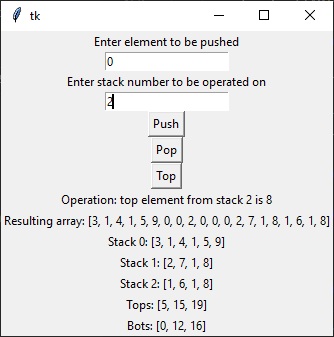
\includegraphics[]{gui}
    \caption{gui}
\end{figure}


\chapter{Tests}
\begin{lstlisting}[language=Python, caption=multistack\_tests.py]
import unittest
from multistack import MultiStack, StackFull, StackEmpty

class TestMultiStack(unittest.TestCase):
    # test creating a small multistack with one stack and array size of 5
    def test_small_single(self):
        ms = MultiStack(1, 5)
        self.assertEqual(ms.is_empty(0), True)
        with self.assertRaises(StackEmpty):
            ms.pop(0)
        ms.push(0, 3)
        self.assertEqual(ms.is_empty(0), False)
        self.assertEqual(ms.top(0), 3)
        ms.pop(0)
        self.assertEqual(ms.is_empty(0), True)
        ms.push(0, 3)
        ms.push(0, 1)
        ms.push(0, 4)
        ms.push(0, 1)
        ms.push(0, 5)
        with self.assertRaises(StackFull):
            ms.push(0, 9)
        self.assertEqual(ms.top(0), 5)
    
    #test creating default multistack with 3 stacks and array size of 20
    def test_default(self):
        ms = MultiStack()
        self.assertEqual(ms.is_empty(0), True)
        with self.assertRaises(StackEmpty):
            ms.pop(0)
        self.assertEqual(ms.is_empty(1), True)
        with self.assertRaises(StackEmpty):
            ms.pop(1)
        self.assertEqual(ms.is_empty(2), True)
        with self.assertRaises(StackEmpty):
            ms.pop(2)
        ms.push(0, 3)
        ms.push(0, 1)
        ms.push(0, 4)
        ms.push(0, 1)
        ms.push(0, 5)
        ms.push(1, 2)
        ms.push(1, 7)
        ms.push(1, 1)
        ms.push(1, 8)
        ms.push(2, 1)
        ms.push(2, 4)
        ms.push(2, 1)
        ms.push(2, 4)
        ms.push(2, 2)
        ms.push(2, 1)
        ms.push(2, 3)
        ms.push(2, 5)
        ms.push(2, 6)
        with self.assertRaises(StackFull):
            ms.push(2, 2)
        self.assertEqual(ms.top(0), 5)
        self.assertEqual(ms.top(1), 8)
        self.assertEqual(ms.top(2), 6)
        ms.pop(2)
        ms.pop(2)
        self.assertEqual(ms.top(2), 3)
        ms.push(0, 9)
        self.assertEqual(ms.top(0), 9)


if __name__ == '__main__':
    unittest.main()
\end{lstlisting}

\chapter{Lessons Learned}
This project seemed simple at first, but once I tried to implement it,
it was much harder than I initially thought. Using an array to store multiple
stacks while dynamically adjusting the gaps between the stacks is very error-prone 
with a lot of very subtle hard to fix bugs.
In class Professor Ammari suggested we use a pointer/linked-list approach to handle
multiple stacks in an array, but that solution would be in conflict with the requirements 
listed in the project through the questions. Although that solution would most likely be much
easier and less error-prone, I decided to follow the project requirements and stick with
a purely array based implementation. I spent a huge amount of time including thinking about 
fixing bugs while eating, showering, and even in my dreams, but when I finally fixed all the bugs 
and got it working, it was extremely satisfying.
The lesson I learned is that sometimes doing things the hard way 
could end up being better than the easy way.

\bibliographystyle{plain}
\bibliography{refs}

% --------------------------------------------------------------
%     You don't have to mess with anything below this line.
% --------------------------------------------------------------
 
\end{document}